% $Id: template.tex 11 2007-04-03 22:25:53Z jpeltier $

%\documentclass{vgtc}                          % final (conference style)
\documentclass[review]{vgtc}                 % review
%\documentclass[widereview]{vgtc}             % wide-spaced review
%\documentclass[preprint]{vgtc}               % preprint
%\documentclass[electronic]{vgtc}             % electronic version

%% Uncomment one of the lines above depending on where your paper is
%% in the conference process. ``review'' and ``widereview'' are for review
%% submission, ``preprint'' is for pre-publication, and the final version
%% doesn't use a specific qualifier. Further, ``electronic'' includes
%% hyperreferences for more convenient online viewing.

%% Please use one of the ``review'' options in combination with the
%% assigned online id (see below) ONLY if your paper uses a double blind
%% review process. Some conferences, like IEEE Vis and InfoVis, have NOT
%% in the past.

%% Figures should be in CMYK or Grey scale format, otherwise, colour 
%% shifting may occur during the printing process.

%% These few lines make a distinction between latex and pdflatex calls and they
%% bring in essential packages for graphics and font handling.
%% Note that due to the \DeclareGraphicsExtensions{} call it is no longer necessary
%% to provide the the path and extension of a graphics file:
%% \includegraphics{diamondrule} is completely sufficient.
%%
\ifpdf%                                % if we use pdflatex
  \pdfoutput=1\relax                   % create PDFs from pdfLaTeX
  \pdfcompresslevel=9                  % PDF Compression
  \pdfoptionpdfminorversion=7          % create PDF 1.7
  \ExecuteOptions{pdftex}
  \usepackage{graphicx}                % allow us to embed graphics files
  \DeclareGraphicsExtensions{.pdf,.png,.jpg,.jpeg} % for pdflatex we expect .pdf, .png, or .jpg files
\else%                                 % else we use pure latex
  \ExecuteOptions{dvips}
  \usepackage{graphicx}                % allow us to embed graphics files
  \DeclareGraphicsExtensions{.eps}     % for pure latex we expect eps files
\fi%

%% it is recomended to use ``\autoref{sec:bla}'' instead of ``Fig.~\ref{sec:bla}''
\graphicspath{{figures/}{pictures/}{images/}{./}} % where to search for the images

\usepackage{microtype}                 % use micro-typography (slightly more compact, better to read)
\PassOptionsToPackage{warn}{textcomp}  % to address font issues with \textrightarrow
\usepackage{textcomp}                  % use better special symbols
\usepackage{mathptmx}                  % use matching math font
\usepackage{times}                     % we use Times as the main font
\renewcommand*\ttdefault{txtt}         % a nicer typewriter font
\usepackage{cite}                      % needed to automatically sort the references
\usepackage{tabu}                      % only used for the table example
\usepackage{booktabs}                  % only used for the table example
%% We encourage the use of mathptmx for consistent usage of times font
%% throughout the proceedings. However, if you encounter conflicts
%% with other math-related packages, you may want to disable it.

%%%%%%%%%%%%%%%%%%%%%%%%%%%%%%%%
\usepackage{hyperref}
\usepackage{cleveref}

\usepackage{graphicx}
\usepackage{subcaption}
\usepackage{xcolor,soul}
\usepackage{tabularx}

\usepackage{url}
\usepackage{amsmath}
\usepackage{algorithm}
\usepackage[noend]{algpseudocode}

\usepackage[labelfont=bf]{subcaption}
\captionsetup{labelfont=bf,textfont=it}

\usepackage{caption}
\usepackage{lipsum}

\algrenewcommand\algorithmicrequire{\textbf{Input:}}
\algrenewcommand\algorithmicensure{\textbf{Output:}}

\def\UrlBigBreaks{\do\/\do-\do:}

\hypersetup{hidelinks=true}

%\newcommand{\nathan}[1] {{\begingroup\sethlcolor{orange}\hl{(nathan:)#1}\endgroup}}
\newcommand{\feng}[1] {\textcolor{blue}{#1}}

%% If you are submitting a paper to a conference for review with a double
%% blind reviewing process, please replace the value ``0'' below with your
%% OnlineID. Otherwise, you may safely leave it at ``0''.
\onlineid{0}

%% declare the category of your paper, only shown in review mode
\vgtccategory{Research}

%% allow for this line if you want the electronic option to work properly
%\vgtcinsertpkg

%% In preprint mode you may define your own headline.
%\preprinttext{To appear in an IEEE VGTC sponsored conference.}



%%%%%%%%%%%%%%%%%%%%%%%%%%%%%%%%%%%

%% In preprint mode you may define your own headline.
%\preprinttext{To appear in an IEEE VGTC sponsored conference.}

%% Paper title.

\title{Interactive Rendering of Large-Scale Volumes on Multi-Core CPUs}

%% This is how authors are specified in the conference style

%% Author and Affiliation (single author).
%%\author{Roy G. Biv\thanks{e-mail: roy.g.biv@aol.com}}
%%\affiliation{\scriptsize Allied Widgets Research}

%% Author and Affiliation (multiple authors with single affiliations).
%%\author{Roy G. Biv\thanks{e-mail: roy.g.biv@aol.com} %
%%\and Ed Grimley\thanks{e-mail:ed.grimley@aol.com} %
%%\and Martha Stewart\thanks{e-mail:martha.stewart@marthastewart.com}}
%%\affiliation{\scriptsize Martha Stewart Enterprises \\ Microsoft Research}

%% Author and Affiliation (multiple authors with multiple affiliations)
\author{Feng Wang\thanks{e-mail: feng@sci.utah.edu}\\ %
	\scriptsize SCI Institute, University of Utah %
\and Ingo Wald\thanks{e-mail: ingowald@gmail.com}\\ %
\scriptsize Intel, Nvidia(Now) %
\and Chris R. Johnson \thanks{e-mail: crj@sci.utah.edu}\\ %
	 \scriptsize \centering SCI Institute, University of Utah}

%% A teaser figure can be included as follows, but is not recommended since
%% the space is now taken up by a full width abstract.
%\teaser{
%  \includegraphics[width=1.5in]{sample.eps}
%  \caption{Lookit! Lookit!}
%}

\teaser{
	\centering
    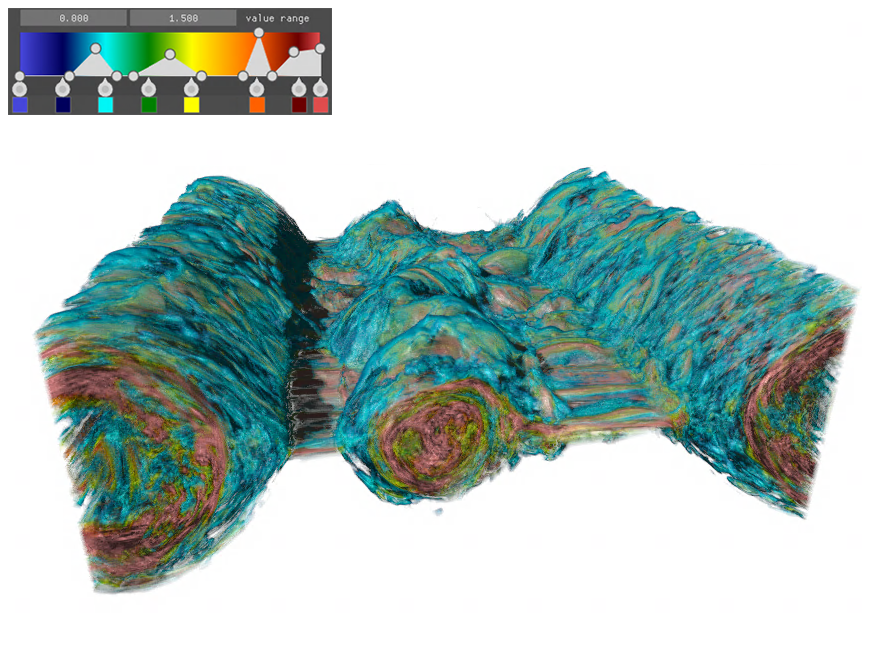
\includegraphics[width=0.3\textwidth]{teaser_1}
    \label{fig:magnetic}
    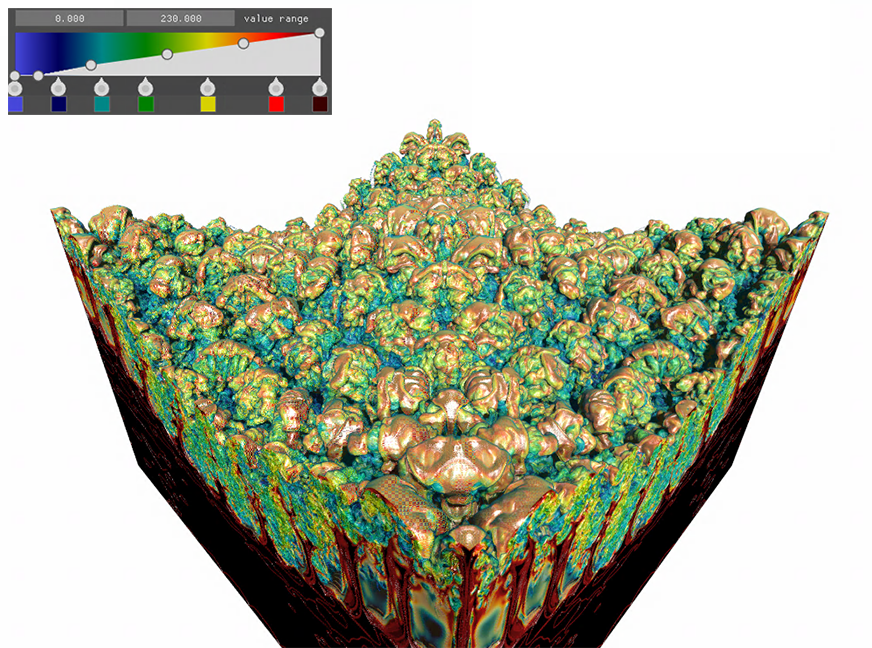
\includegraphics[width=0.3\textwidth]{teaser_2}
    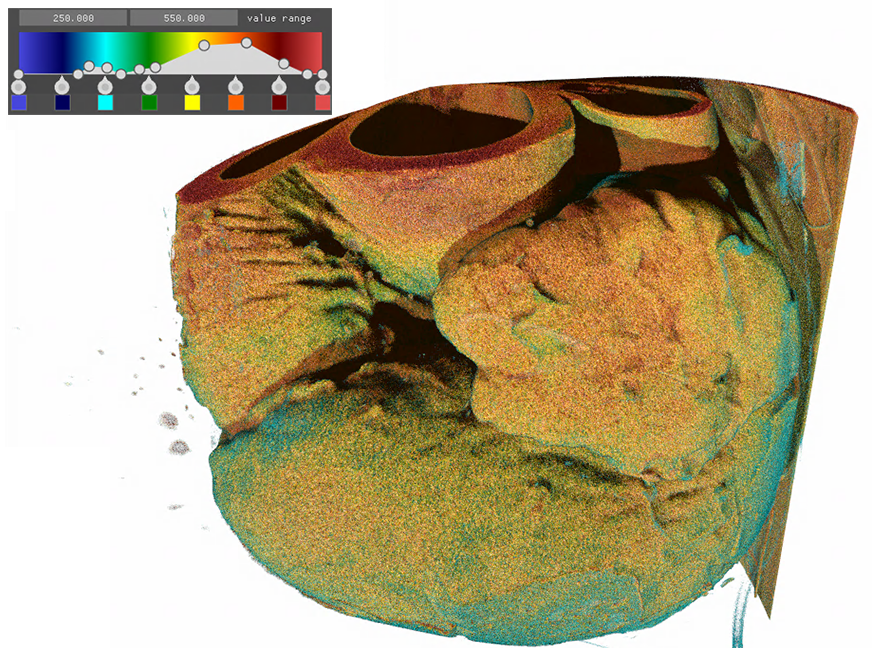
\includegraphics[width=0.3\textwidth]{teaser_3}
    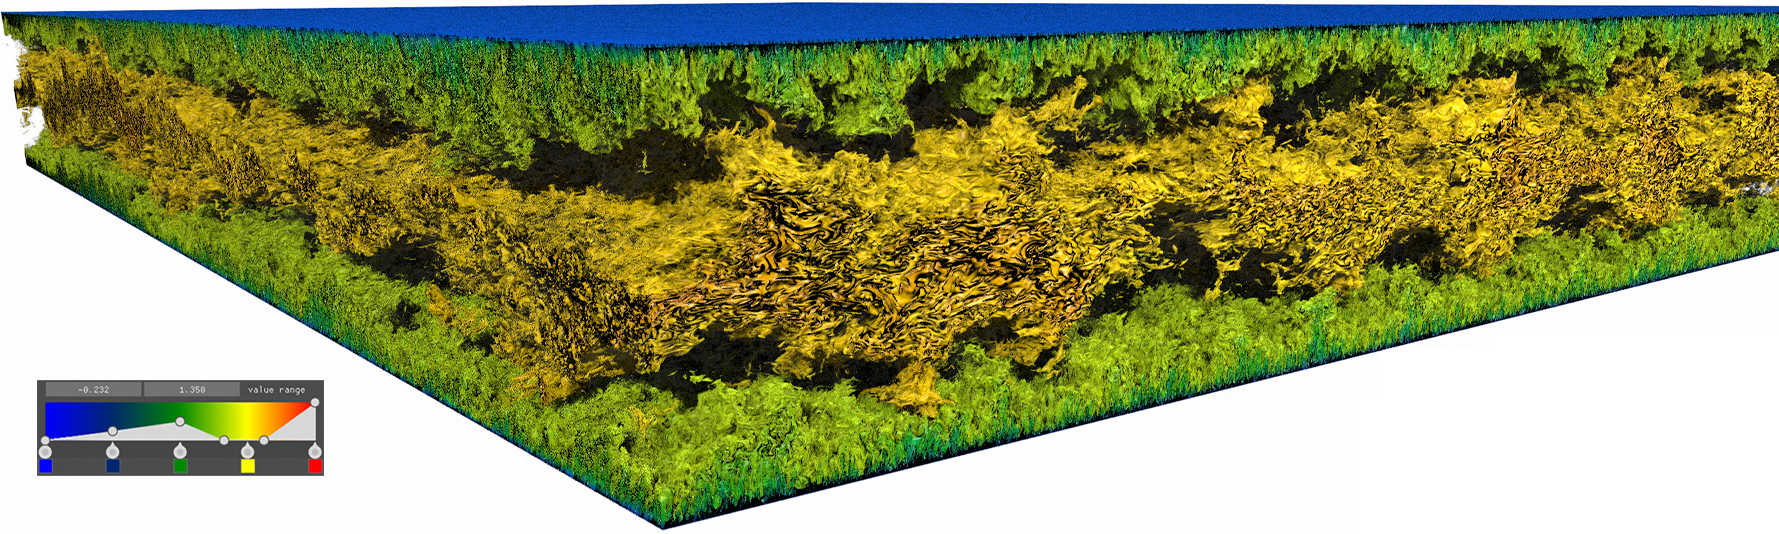
\includegraphics[width=0.9\textwidth]{teaser_4}
    %\captionsetup{width=0.85\textwidth}
	\caption{\label{fig:teaser}Screenshots from our high-fidelity interactive volume visualization renderer. Top left: volume rendering of a $512^3$ magnetic reconnection dataset~\cite{guo2014formation}. Top middle: volume rendering of the $2048\times 2048\times 1920$ Richtmyer-Meshkov instability (RMI)~\cite{cohen2002three}. Top right: visualization of a $2048\times 2048\times 2612$ cardiac volume~\cite{scivisdata}. Bottom: visualization of the $10240\times 7680\times 1356$ DNS dataset~\cite{moser1999direct}. All images are rendered with surface shading.}
}


%% Abstract section.
\abstract{Recent advances in large-scale simulations have resulted in volume data of increasing size that stress the capabilities of off-the-shelf visualization tools. Users suffer from long data loading times, because large data must be read from disk into memory prior to rendering the first frame. In this work, we present a volume renderer that enables high-fidelity interactive visualization of large volumes on multi-core CPU architectures. Compared to existing CPU-based visualization frameworks, which take minutes or hours for data loading, our renderer allows users to get a data overview in seconds. Using a hierarchical representation of raw volumes and ray-guided streaming, we reduce the data loading time dramatically and improve the user's interactivity experience. We also examine system design choices with respect to performance and scalability. Specifically, we evaluate the hierarchy generation time, which has been ignored in most prior work, but which can become a significant bottleneck as data scales. Finally, we create a module on top of the OSPRay ray tracing framework that is ready to be integrated into general-purpose visualization frameworks such as Paraview.} % end of abstract

%% ACM Computing Classification System (CCS). 
%% See <http://www.acm.org/about/class> for details.
%% We recommend the 2012 system <http://www.acm.org/about/class/class/2012>
%% For the 2012 system use the ``\CCScatTwelve'' which command takes four arguments.
%% The 1998 system <http://www.acm.org/about/class/class/2012> is still possible
%% For the 1998 system use the ``\CCScat'' which command takes four arguments.
%% In both cases the last two arguments (1998) or last three (2012) can be empty.

\CCScatlist{
  \CCScatTwelve{Human-centered computing}{Visu\-al\-iza\-tion}{Visu\-al\-iza\-tion techniques}{Treemaps};
  \CCScatTwelve{Human-centered computing}{Visu\-al\-iza\-tion}{Visualization design and evaluation methods}{}
}

%\CCScatlist{
  %\CCScat{H.5.2}{User Interfaces}{User Interfaces}{Graphical user interfaces (GUI)}{};
  %\CCScat{H.5.m}{Information Interfaces and Presentation}{Miscellaneous}{}{}
%}

%% Copyright space is enabled by default as required by guidelines.
%% It is disabled by the 'review' option or via the following command:
% \nocopyrightspace



%\author[F. Wang \& I. Wald \& C. R. Johnson]
% {\parbox{\textwidth}{\centering F. Wang$^{1}$, I. Wald$^{2}$ and C. R. Johnson$^{1}$
% \vspace*{-0.5cm}
% 		%\orcid{0000-0001-7756-0901}
% %        and S. Behnke$^{2}$\orcid{0000-0001-5923-423X} 
% %        S. Spencer$^2$\thanks{Chairman Siggraph Publications Board}  
%         }
%         \\
% % For Computer Graphics Forum: Please use the abbreviation of your first name.
% {\parbox{\textwidth}{\centering $^1$SCI Institute, University of Utah\\
%          $^2$ Nvidia Corporation.
% %        $^2$ Another Department to illustrate the use in papers from authors
% %             with different affiliations
%       } 
% }
% \vspace*{-3em}
%}


% ------------------------------------------------------------------------

% if the Editors-in-Chief have given you the data, you may uncomment
% the following five lines and insert it here
%
% \volume{27}   % the volume in which the issue will be published;
% \issue{1}     % the issue number of the publication
% \pStartPage{1}      % set starting page

%%%%%%%%%%%%%%%%%%%%%%%%%%%%%%%%%%%


% For backwards compatibility to old LaTeX type font selection.
% Uncomment if your document adheres to LaTeX2e recommendations.
% \let\rm=\rmfamily    \let\sf=\sffamily    \let\tt=\ttfamily
% \let\it=\itshape     \let\sl=\slshape     \let\sc=\scshape
% \let\bf=\bfseries

% end of prologue


%-------------------------------------------------------------------------
\begin{document}

\maketitle

%-------------------------------------------------------------------------
\section{Introduction}
\label{sec:introduction}
Interactive visualization of large-scale volumetric data, produced by
simulations, astronomical instruments and high-resolution sensors, 
allows research scientists to explore scientific data, validate
hypotheses and discover new knowledge~\cite{keim2013big}. 
However, the increasing data resolution in current high-performance
computing (HPC) simulations can easily surpass the capabilities of
host systems, making interactive visualization of such data challenging. 
First, loading the full-resolution data into main memory is impractical
due to memory limitations. Second, for large datasets, the IO latency incurred by the data 
loading process is prohibitive in the existing volume renderer,
even if all the data fit into memory.
The long IO waiting time for large dataset degrades the user experience.
Therefore, research on novel techniques for
data visualization, processing, storage and IO that scale to 
extreme-scale data is required to transcend the limitations
of current hardware~\cite{beyer2014survey}.



Current solutions for scalable volume data visualization mostly employ GPU architecture,
since it has been shown to be effective for interactive visualization. 
Prior studies~\cite{crassin2009gigavoxels,engel2011cera,hadwiger2008interactive} 
have applied out-of-core approaches, level-of-detail (LOD) techniques,
progressive rendering and data compression schemes to overcome GPU memory limitations. 
However, these approaches inevitably employ extra data structures (e.g., page tables)
and incur frequent CPU-GPU communication to refine the visible data, which hampers the interactivity. Some studies also consider architectures employing CPUs, since the amount 
of memory directly accessible by a CPU often dwarfs the amount of VRAM available on even
the most powerful GPUs. Previous studies have shown that an optimized CPU volume renderer 
can outperform a GPU renderer for sufficiently large volumes ~\cite{smelyanskiy2009,knoll2011full,wald2017ospray}. However, several studies~\cite{childs2006scalable,peterka2008parallel,howison2012hybrid}
have focused on distributed parallel rendering on supercomputers, but very few have addressed interactive visualization of large-scale volumes on a single workstation.



% Due to their efficient built-in texture interpolation, GPUs have been shown to be 
% effective for interactive visualization of moderate-size volume data. 
% For large-scale datasets, 
% prior studies~\cite{crassin2009gigavoxels,engel2011cera,hadwiger2008interactive} 
% have applied out-of-core approaches, level-of-detail (LOD) techniques and
% progressive rendering to overcome GPU memory limitations. 
% However, these approaches inevitably employ extra data structures (e.g., \textcolor{blue}{page tables})
% and incur frequent CPU-GPU communication to perform visibility calculations
% and data refinement. 


% Furthermore, most of these approaches are project-specific and have not been 
% integrated into general-purpose visualization frameworks, and are thus not widely used. 

% Multi-core CPUs are a desirable platform
% for large-scale volume rendering for many reasons~\cite{knoll2011full}. The amount of
% memory directly accessible by a CPU often dwarfs the amount of VRAM
% available on even the most powerful GPUs. Previous studies have shown that an
% optimized CPU volume renderer can outperform a GPU renderer
% for sufficiently large volumes ~\cite{knoll2011full,smelyanskiy2009}.
% For purely CPU-based large-scale volume rendering systems, much 
% research~\cite{childs2006scalable,peterka2008parallel,howison2012hybrid}
% has been done on distributed parallel rendering on supercomputers. 
% However, very few previous papers have focused on interactive visualization of
% large-scale volumes on a single workstation. Furthermore, the 
% aforementioned general-purpose frameworks struggle to
% perform well on large-scale data. 

In this work, we present an interactive visualization solution for large-scale
volumes on multi-core CPU architectures. Our solution allows users to get an overview of the large
data in seconds rather than minutes or hours using existing visualization frameworks. 
We build our approach on a hierarchical data structure -- \textit{Bricktree} -- that allows
for a hierarchical representation of the volume. During the rendering, we stream the
necessary data on demand with separate threads and employ ray-guided progressive
rendering for data refinement. As an extension of the OSPRay ray tracing 
framework, which already contains various techniques for visualizing scientific data \cite{wald2017ospray,wang2018cpu}, we build a Bricktree
module along with an efficient hierarchy generation tool to support large-scale data
visualization on multi-core workstations. Given that OSPRay has been integrated into
Paraview and VisIt, our module is ready to be integrated into general-purpose
visualization frameworks. Specifically, our contributions in this paper are:

\begin{itemize}
\item An interactive visualization solution for large-scale volume
visualization, which decouples the data loading and rendering process 
on multi-core architectures and dramatically reduces the amount of time the user has to
wait before being able to explore the data. 
\item The Bricktree, an efficient and low-overhead hierarchical structure that
allows for encoding a large volume into a multi-resolution representation.
We also evaluate the structure with several choices of parameters. 
\item An OSPRay module for large data visualization
and a parallel hierarchy generation tool that are ready to be 
"dropped into" a general-purpose visualization pipeline.  
\end{itemize}



%-------------------------------------------------------------------------
\section{Previous Work}

Although widely used for visualization of 3D scalar fields, volume rendering
remains a computation, memory and I/O-intensive task~\cite{wu2018visit}. 
Several studies have focused on improving the rendering performance by
introducing efficient packet BVH traversal~\cite{knoll2011full,wald2017ospray}, 
empty space skipping~\cite{hadwiger2018sparseleap} and
early ray termination~\cite{levoy1990efficient,kruger2003acceleration}.
Although efficient for visualizing moderate-size volumes on consumer desktops, 
these methods struggle to scale to petascale or exascale datasets, since they assume that the entire volume is present in memory. 
% these methods 
% assume that the entire volume is present in memory and struggle to scale
% to petascale or exascale datasets.
Previous work on large-scale volume rendering
can be categorized as: 

1) Parallel/distributed rendering on distributed memory systems. These approaches
parallelize data processing over many nodes~\cite{childs2010extreme}. Research
has demonstrated strong scalability on both CPU and GPU clusters~\cite{childs2006scalable,
howison2012hybrid,peterka2008parallel,eilemann2009equalizer,fogal2010large,beyer2011distributed}. 
For example, Howison et al.~\cite{howison2012hybrid} demonstrated that MPI-hybrid
parallelism achieves a sublinear raycasting speed-up and is more efficient in terms of
overall speed and memory than the MPI-only parallelism.
However, previous work~\cite{wu2018visit} has found that the main
performance bottleneck of distributed visualization lies in final image compositing
rather than in the volume rendering process.

2) Visualization of large-scale volumes on a stand-alone workstation.
Much effort has been devoted to the implementation of GPU renderers
due to the great hardware interpolation capabilities\cite{feng2015parallel,clyne2007interactive}.
Beyer et al.~\cite{beyer2014survey} conducted a detailed survey on this topic. Most prior work focuses on overcoming the GPU's
memory limitation and tackling this issue by loading only the visible
part of the volume into GPU memory~\cite{li2003empty}. 
The GigaVoxels system~\cite{crassin2007interactive,crassin2009gigavoxels}, the first to employ this idea, determines the visibility of
small blocks ``on the fly''.  
Although capable of rendering several billion voxels in real-time,
it mainly focuses on entertainment applications and targets sparse volume datasets.
CERA-TVR~\cite{engel2011cera} then extended the GigaVoxel paper, 
targeting scientific visualization user cases.
In contrast to GigaVoxel, CERA-TVR is capable of rendering dense volumes
and can progressively refine parts of a framebuffer if the size of the visible
data exceeds the size of the brick pool.
Hadwiger et al.~\cite{hadwiger2012interactive} proposed a virtual memory scheme
that avoids explicit tree traversal and supports interactive visualization and 
streaming of petascale 2D image data. However, this approach exhibits
IO latency during 3D block construction due to cache misses and requires that all
visible data fit into cache. All these approaches inevitably require
heavy CPU-GPU communication, which significantly impacts interactivity. 


In the context of the CPU-based renderers, very little research has focused
on large-scale volume rendering on multi-core workstations.
As a state-of-art CPU ray-tracing framework for scientific visualization,
OSPRay works well for interactive visualization of moderate-size volume data
and can potentially be extended to large-scale data.
Wu et al.~\cite{wu2018visit} proposed the VisIt-OSPRay system, which can scale to
large-scale datasets. To achieve interactive visualization, they integrated OSPRay
into VisIt as a backend visualization toolkit and coupled it with PIDX (parallel IO 
library)~\cite{kumar2011pidx} for scalable IO. 
This study achieved interactive visualization, but it took more than 30 minutes to load the DNS 
dataset into memory with 64 processors on Stampede2.
%(a supercomputer at the Texas Advanced Computing Center (TACC)). 

To address these challenges, we decompose large volumes into a hierarchical 
representation, with each node representing a small cubic brick. Within the rendering pipeline,
we leverage ray-guided streaming and progressive rendering to reduce IO latency.


%-------------------------------------------------------------------------
\section{Bricktrees}

\feng{Adaptive space subdivision and hierarchical data representation are
key to interactive visualization of large-scale volumetric datasets\cite{crassin2009gigavoxels}.
These techniques enable us to load and update the working set on demand to address IO latency
and memory limitations. As a popular hierarchical data structure for 3D space subdivision,
the octree has been well studied for direct volume rendering\cite{gobbetti2008single}.
Hierarchical grids feature a theoretically optimal number of traversal steps,
and thus have been adopted as general-purpose ray-tracing acceleration structures
\cite{knoll2006interactive}. Lefebvre et al.\cite{lefebvre2005octree} proposed
the $N^3$-tree, which is capable of decomposing a node by an arbitrary number $N^3$ and
has a branching factor of $N^3$.
The GigaVoxel system \cite{crassin2009gigavoxels} also use a hierarchical data structure
that is similar to the $N^3$-tree, but has a smaller branching factor of $2^3$ (as shown in
\Cref{fig:tree_comparision}).
Other structures, such as kd-trees, have also been used in isosurface rendering with
the trend of coherent ray tracing\cite{wald2001interactive,procopiuc2003bkd,wald2005faster}. 
}

\begin{figure}[h]
  \centering
  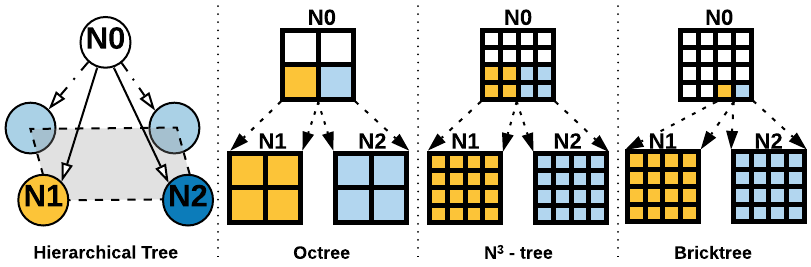
\includegraphics[width=\columnwidth]{tree_comparision}
  \caption{\label{fig:tree_comparision}Comparison of the data structure with an octree, the GigaVoxel's hierarchy and an $N^3$-tree (Bricktree) in 2D representation.
  In a 3D scenario, an octree has a branching factor of $2^3$ and allows for decomposing a node into $2^3$ cells; an $N^3$-tree has a branching factor
  of $2^3$ and allows for decomposing a node into $N^3$ cells; a Bricktree has a branching factor of $N^3$ and allows for
  decomposing a node into $N^3$ cells.}
    %\vspace{-1em}
\end{figure}


\begin{figure*}[h]
  \centering
    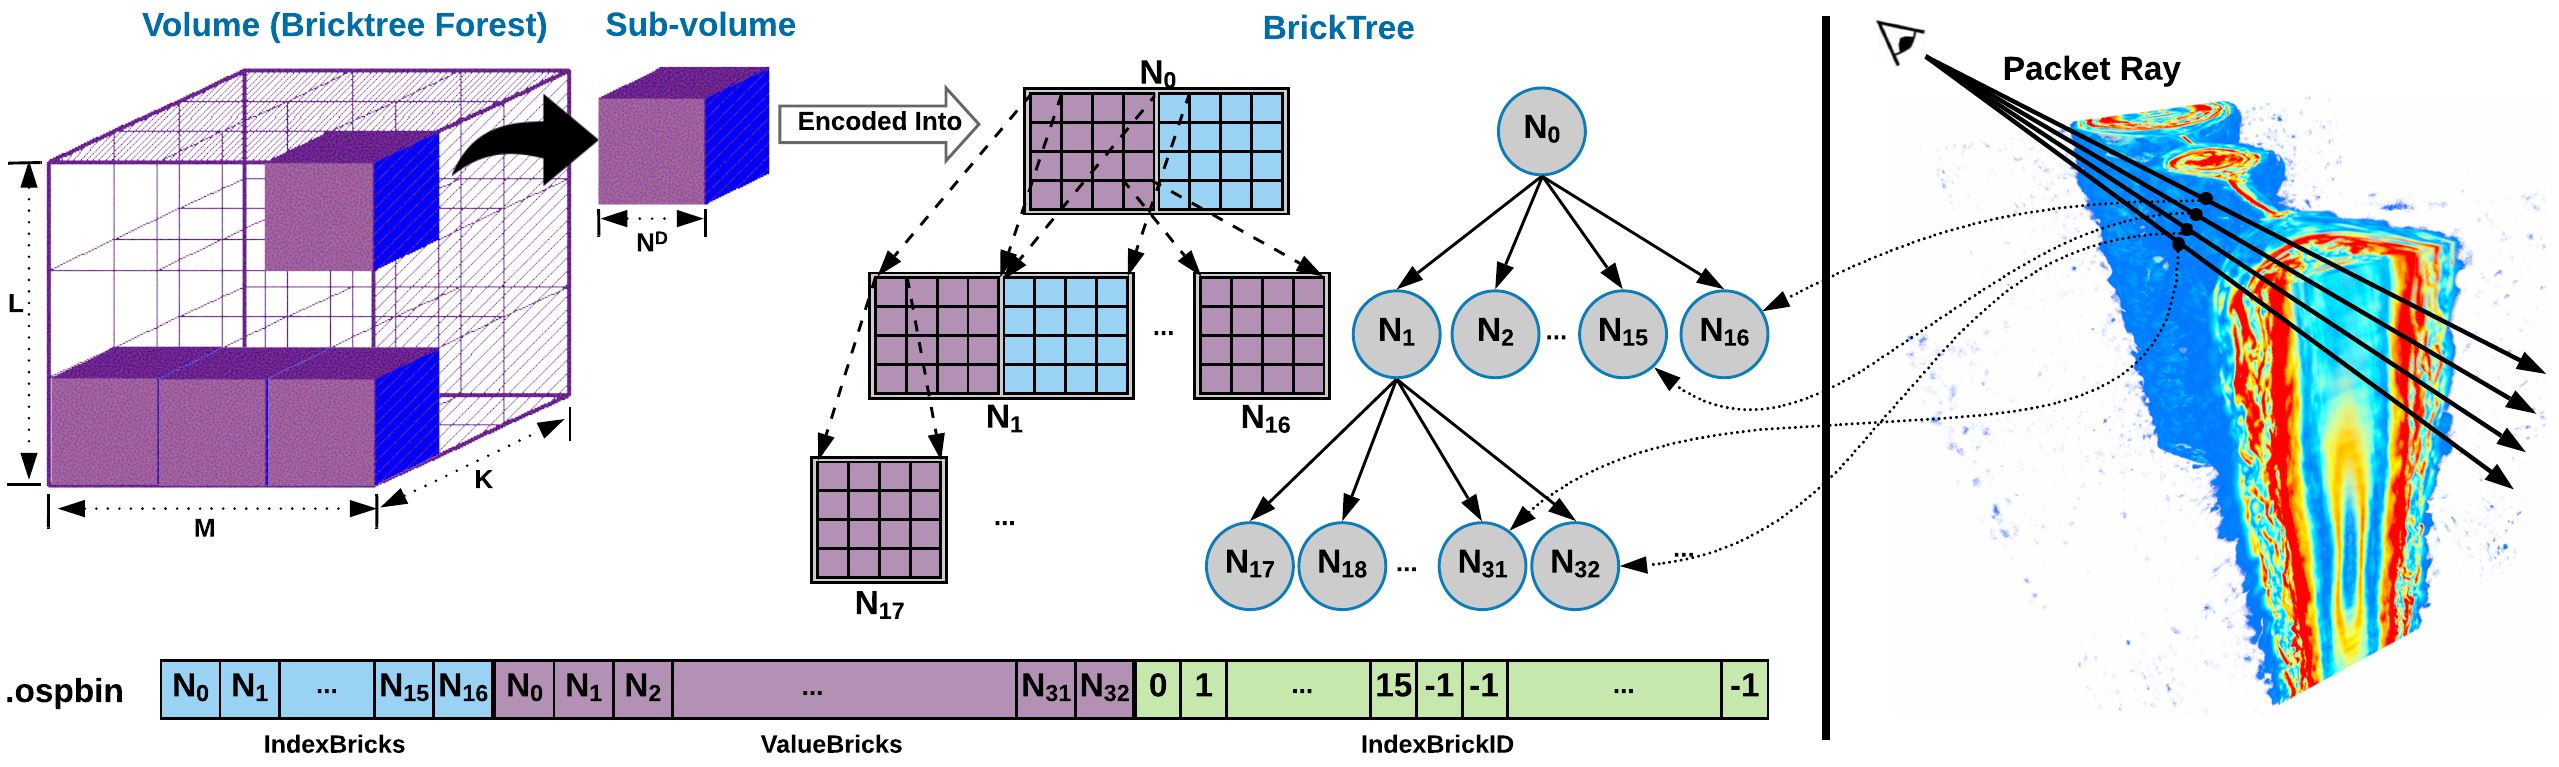
\includegraphics[width=0.99\textwidth]{BricktreeLayout}
	\caption{\label{fig:bricktree_layout}An illustration of the layout of the Bricktree structure. Each brick (e.g. $N_0,N_1 ...$) is represented with a Valuebrick (colored in purple), an indexBrickID and an optional Indexbrick (colored in light blue). The indexBrickID stores the index of the Indexbrick if a node has one. Otherwise, -1 is stored. Both Valuebricks and Indexbricks contain $N^3$ cells. 
Each cell encodes a float value in a Valuebrick or an int32 reference in an Indexbrick.}
    %\vspace{-1em}
\end{figure*}


\feng{
In this work, we define a hierarchical data structure --``Bricktree''-- that allows
us to represent a structured volume in a hierarchical, multi-resolution and compressed
way (as shown in \Cref{fig:bricktree_layout}).
Rather than encoding the large volume into a single deep Bricktree, our design
tiles the volume into a ``Bricktree Forest'', which consists of a list of Bricktrees.
By encoding a sub-volume into a Bricktree, we guarantee that using a 32-bit int
can safely refers to all the bricks. 
This design not only is conducive to parallel tree traversal on multi-core CPU architectures,
but also avoids encoding a large empty space when the structured volume is not a perfect
cube ($M \neq L \neq K $).
Overall, a Bricktree is a generalization of an octree where we subdivide a node by $N^3$
rather than by $2^3$. Furthermore, a Bricktree is similar with the $N^3$-tree on data struture,
but different on data layout in memory. Each cell in an $N^3$-tree node either stores a data
value or an reference to the children, whereas in a Bricktree node always store a data value. 
In a Bricktree, we intentionally store the value and reference in seperate buffers so that we could 
save memory by storing only one invalid reference for a brick if none cell in this brick have
children, 
rather than storing $N^3$ invalid references with one for each cell in an $N^3$-tree. 
A detail introduction about the layout of Bricktree is described in the next section. 
}


%-------------------------------
\subsection{Data Layout}
\label{sec:bricktree_layout}

\feng{
In our design, a ``brick'' is an $N \times N \times N$ set of cells. Obviously, each cell can
store a data value. We denote a brick that stores data values as a ``Valuebrick''. Bricks can
be thought of as nodes of a tree with branching factor $N^3$. We call such a tree a ``Bricktree''.
Each brick can have up to $N^3$ children, where each child brick is associated with exactly one
cell in the parent brick. If a brick does have children, the child indices are stored in an 
``Indexbrick''. Thus, we represent a brick as a Valuebrick and an optional Indexbrick in memory 
and also along with an indexBrickID to indicate the corresponding relationship between the Valuebrick
and the Indexbrick.
}

\feng{
Each cell of a Valuebrick corresponds to a set of voxels in the volume. For a ``leaf brick''
(e.g., $N_{16}$), one cell corresponds to exactly one voxel, and the cell's value equals the
value of this voxel. By contrast, each cell of an ``inner brick'' (e.g., $N_0$) typically
represents a set of voxels. Accordingly, we can assign a value to each cell. How to calculate 
this value is totally your choice. In our implementation, we compute this value by averaging
over all voxels in this set. Each cell of an Indexbrick refers to a child brick if the current
brick has children. A ``leaf brick'' has no children and thus no Indexbrick. In this
case, the indexBrickID of this brick is set to invalid (-1), whereas for an ``inner brick'', its
indexbrickID refers to the right Indexbrick, and the cells in this Indexbrick point to the children.
In \Cref{fig:bricktree_layout}, a Valuebrick is shown in purple and an Indexbrick is in light blue. 
}

\feng{
Multiple Bricktrees can be combined to form a ``Bricktree Forest''. Recall that this allows us
to tile a nonsquare domain efficiently. \Cref{fig:bricktree_layout} (left) illustrates a structured
volume with dimension $M \times L \times K$, which is organized into a Bricktree Forest.
Each Bricktree is specified through a brick size (N), a data type (T) and a tree depth (D), and 
represents a set of $N^D \times N^D \times N^D$ voxels in the volume. 
}


%\feng{
%Each cell in an indexbrick can -- but is not required to -- refer to a child brick with a child index.
%The child indices are encoded through two level of indirection: first, if a brick don't have an indexbrick
%or the indexbrickID is marked as invalid, then none of the brick's cells have children; If the brick have
%an indexbrick, we further check the child index that is stored in the indexbrick's cell. The child index 
%indicates the location of the child brick. A given cell does not have children when its corresponding
%child index is marked as invalid. 
%}


In memory, each $BrickTree<N,T>$ is represented as three linear arrays:
\begin{enumerate}
\item One linear array of Valuebricks, where each Valuebrick contains
$N \times N \times N$ values of type T.
\item One linear array of int32 ``indexbrickIDs'', with exactly one such
int32 per Valuebrick. If a given Valuebrick's indexbrickID is -1,
it does not refer to an Indexbrick and thus none cell in the brick has children;
otherwise, this ID refers to an Indexbrick in the Indexbrick array.
\item One linear array of ``Indexbricks``, where each Indexbrick contains
$N \times N \times N$ int32 indices. Each such index can be -1 (meaning the
corresponding cell does not have a child); 
if the index is greater than or equal to 0, it refers to a brick in the Valuebrick array.
% (which in turn can have childrenreferred to it's index brick ID, etc).
\end{enumerate}

\feng{
On a file system, the whole volume is represented by three types of files:
1) one high-level file in XML format that contains meta-data ($N,T, (M,L,K)$ of input volume, etc.)
and represents the Bricktree Forest; 
2) one XML file for each Bricktree that gives high-level information ($N, T, D$, etc.) of the current
bricktree. 
3) one binary file for each Bricktree that stores the three buffers (Valuebricks, Indexbricks and indexbrickIDs). 
}


%----------------------------------
\subsection{Bricktree Overhead}
Due to the specific layout, our Bricktree is easy to index and the overhead is low. 
Given a Bricktree with a brick size of 4, a data type of float and a depth of 4 ($Bricktree<4,float>$), a certain number of $4^3$ Valuebricks and $4^3$ Indexbricks will be generated when building the tree.
In practice, leaf Valuebricks have zero overhead, since each costs 
exactly 256 bytes for 64 float-type cells. The only overhead lies in the 
Indexbricks and inner Valuebricks. However, few of these bricks exist relative
to the number of leaf bricks (see  \Cref{fig:loadbylevel}).

\feng{
In a more ideal case, where many of the inner 
nodes all point to the leaf Valuebrick, we store only about one 32-bit int (4~byte)
for a complete leaf Valuebrick. Hence, 4~bytes are used to index 256 ``payload''
bytes for float data. A less ideal case is that some children of inner nodes are leaves,
whereas other children are inner nodes. Recall that for each inner node, we need to store 
both a Valuebrick and an Indexbrick, which will result in more memory consumption than in the ideal case.
However, the overhead will still most likely be considerably less than that of an octree. 
Benchmarks in \Cref{table:brick_size} show that the in-memory size of a Bricktree with $N = 4$
is much smaller than a Bricktree with $N = 2$, which is an octree. 
In addition, few bricks are located in the upper levels of the tree. Assuming a brick
size of 4, the number of inner nodes goes down by a factor of 64 each time we go up one level
in the tree. This holds in practice - the overhead of Bricktree with $N=4$ is 8.0\% on
the magnetic reconnection dataset (see \Cref{fig:exp_threshold_2}) and the DNS dataset
(see \Cref{table:brick_size}). By contrast, the overhead of an octree (Bricktree with $N=2$) that is built on top of those data is 43\% 
and 72\%, respectively. 
}

%----------------------------------
\subsection{Hierarchy Generation in Parallel}
\label{sec:hierarchy_generation}

As an offline process that is usually run in advance, the performance of reorganizing the volume
into multi-resolution bricks is mostly ignored in the volume rendering literature\cite{fogal2013analysis}. However, the performance becomes a significant
bottleneck for large-scale datasets. Fogal et al. reported that
the runtime for building a hierarchical structure for RMI (8.1~GB, 
$2048 \times 2048 \times 1920$) is up to 1.5 hours in the worst case and
13 minutes in the best case \cite{fogal2013analysis}.
Petascale datasets might take hours or days. 
The virtual memory architecture of \cite{hadwiger2012interactive} alleviates this
problem by constructing the brick at runtime. However, the latency of constructing
bricks at runtime will dramatically influence the framerate, especially when the 
visible data are missing in memory. 

\feng{
Our design also makes hierarchy generation more efficient. 
It is straightforward to construct the Bricktree Forest in parallel.
Rather than parallelizing the process using $tbb::parallel\_for$, 
our ``\textit{ospRawToBricks}'' tool employs the \textit{GNU make} command to meet the end.
This choice benefits us to specify a customized number of trees to build in parallel in case
that we consumer all the host memory. 
Normally, \textit{make} will execute only one recipe at a time.
By specifying the ``\textit{-j}'' option, it is possible to execute many recipes simultaneously.
Once parameters $N$, $T$ and $D$ are set, we first generate an index file over the Bricktrees
as well as a makefile. The makefile is used to build each Bricktree in parallel.
\Cref{alg:bricktree} shows the algorithm for recursively constructing a Bricktree. 
Measurements of the performance improvement from parallelization are shown in
\Cref{fig:exp_buildtime}.
}


\begin{algorithm}
	\caption{The recursive function for constructing a Bricktree. $N,T$ is defined as template parameters. $Threshold$ is a customized parameter for ``compression''.}\label{alg:bricktree}
	%\hspace*{\algorithmicindent} \textbf{Input} \\
    %\hspace*{\algorithmicindent} \textbf{Output} 
	\begin{algorithmic}[1]
	    \Require $llC$ - left lower coord; $lvl$ - tree level; $lvlWidth$ - level width.
        \Ensure $avgValue$ - average value of a brick; $vRange$ - value range.
		\Function{BuildRec}{$avgValue, llC, lvl, lvlWidth$}
			\State $cellSize \gets lvlWidth / N $
			\State $brick, vRange$
			\If {levelWidth ==  N}
				\State $brick.value[i][j][k] \gets input.get(N * llC + offset)$
				\State $vRange.extend(brick.value[i][j][k])$
			\Else
			    \State $lowerLeft \gets N*llC + offset$
				\State $vRange \gets BuildRec(avg,lowerLeft, lvl+1,cellSize))$
				\State $brick.value[i][j][k] \gets (T)avg$
			\EndIf
			\State $avgValue \gets brick.ComputeWeightedAverage()$
			\If{$vRange \leq threshold$}
				\State \textit{This is a brick with each cell of same value.}
				\State \textit{Kill this brick (value has been saved in parent node).}
			\Else
				\State \textit{Set this brick into the brick buffer.}
			\EndIf
			\Return $vRange$
    	\EndFunction
	\end{algorithmic}
\end{algorithm}



%One advantage of constructing a bricktree forest is that the hierarchy 
%generation process can be executed in parallel. The ``\textit{ospRawToBricks}''
%tool, which employs the \textit{GNU make} command, is used to meet this end.
%Normally, \textit{make} will execute only one recipe at a time.
%By specifying the ``\textit{-j}'' option, it is possible to execute many recipes
%simultaneously.
%Once parameters $N$, $T$ and $D$ are set, we first generate the index file of blocks
%as well as a makefile, which will then be used to build each block of the
%bricktree forest. 

\feng{
In addition, our tree construction approach also supports data format conversion and compression.  
We can easily convert an input data format to an interval format, such as double to float. 
Furthermore, we allow the user to set a threshold ($t$) that determines which input regions
can be safely collapsed into a single node. For instance, consider a cell $C$ with a child brick $B$.
Let $Value(b)$ be a function that obtains the value at cell $b \in B$ and $t$ be the threshold:}

\begin{equation} \label{eq:collapse_thresh}
\left(\max_{b \in B} Value(b)\right) - \left(\min_{b \in B} Value(b)\right) \leq t
\end{equation}

\feng{
If Equation \ref{eq:collapse_thresh} holds, then $B$ and its children are ``collapsed'' into $C$, meaning that $C$ no longer points to a child brick, and is instead assigned the average value of all cells in $B$. Our default value of $t$ is 0, meaning that by default, our implementation losslessly eliminates equal-value regions.}


%-------------------------------------------------------------------------
\section{Volume Integration}
In this section, we illustrate the rendering pipeline with Bricktrees in a
simple case where all data have been read into memory.  
Raycasting-based volume rendering consists of marching rays through the volume with
a step size and accumulating color and opacity along the ray. With a hierarchical
structure, rays need to traverse the structure until reaching a leaf node, an inner
node with an appropriate level-of-detail in current viewport or an unmapped node. 

% In contrast to hierarchical structures provided by current GPU-based approaches 
% \cite{crassin2009gigavoxels, hadwiger2012interactive},
% the CPU allows for greater control over these structures\cite{knoll2006interactive}.

\begin{algorithm}
	\caption{Pseudocode on sampling a given point $p$ and traversal of the Bricktree structure }\label{alg:sample}
	\begin{algorithmic}[1]
		\Function {Bt\_Cplus\_Sample}{$p$}
        	\State $vArray[8]\gets \textit{0}$
            \State $\textit{voxelCoord[8]} \gets \textit{Calculate 8 vertex's coordinates}$
            \While{$i < 8$}
            	\State $bTreeID \gets ComputeBrickTreeID(voxelCoord[i])$
                \State $bt \gets GetBrickTree(bTreeID)$
            	\State $vArray[i] \gets Bt\_Cplus\_GetVoxels(bt,voxelCoord[i])$
            \EndWhile
            \State $result \gets lerp(vArray[8])$
            \State \Return $result$
    	\EndFunction
        \Function {Bt\_Cplus\_GetVoxels}{$bt, coord$}
        	\State $brickID\gets \textit{0}$\Comment{top-down traversal}
            \State $brickStack.push(brickID)$
            \While{brickStack is not empty}
            	\State $cBrickID \gets brickStack.pop()$
                \State $ibID \gets bt.brickInfo[cBrickID].indexBrickID$
            	\State $cOffset \gets ComputeOffset(coord)$
                \State $childBrickID \gets bt.indexBrick[ibID].child[cOffset]$
                \If {$childBrickID = -1$} 
                	\State \Return $bt.valueBrick[cBrickID].child[cOffset]$
                \Else
                	\State $brickStack.push(childBrickID)$
                \EndIf
            \EndWhile
    	\EndFunction
	\end{algorithmic}
\end{algorithm}

%Now we describe bricktree traversal on the many-core CPUs. 
For a given sample point $p$ along a ray, we need to query the value of eight
neighboring voxels for interpolation. For each voxel, a tree traversal
is needed to fetch the Valuebrick that the voxel belongs to. We start the Bricktree
traversal from the root node. Assume that we operate on brick 1 of a 
$BrickTree<4,float>$ and want to know if its cell $(1,1,2)$ has a child.
First, we look up the brick's index brick ID ($ibID = indexBrickID[1]$).
We know that none of the cells of brick 1 have a child if the $ibID$
is invalid or less than 0. If this is the case, cell $(1,1,2)$ certainly does not have a child.
However, if $ibID \geq 0$ (e.g., $ibID = 1$ in \autoref{fig:bricktree_layout}), 
then we look at $cellChildID = IndexBrick[ibID].child[1][1][2]$. 
If this value is invalid (-1), then this particular cell of brick 1 does not have any
children. Otherwise, $valueBrick[cellChildID]$ is the child brick.

Algorithm \ref{alg:sample} describes the general sampling process. 
Trilinear interpolation of the eight-nodal value is used to determine the value of an 
arbitrary point $p$. $Bt\_Cplus\_GetVoxels$ traverses the Bricktree and queries the 
value of a given cell. 

So far, we have obtained a sample kernel that has access to the Bricktree ``forest'' and is 
implemented with C++ code. However, as a loadable module to the OSPRay ray tracing
framework, our Bricktree module employs the OSPRay rendering pipeline, which is internally
built on top of Embree\cite{wald2014embree} and ISPC\cite{pharr2012ispc}. Embree is
a collection of high-performance ray tracing kernels. 
The Intel SPMD Program Compiler (ISPC) allows a number of program instances
to execute in parallel on SIMD hardware. ISPC compiles its own programming language
(a variant of C), and this ISPC code can call and be called from C/C++ application code.
In OSPRay, the sampling process maps well to the SIMD paradigm, and is thus implemented
with ISPC code. Under this condition, we can have two approaches to implement our
sampling process. 



%----------------------------------
\subsection{C/C++ Serial Implementation}

A simple but inefficient approach is a serial implementation with C/C++ code without
maintaining a copy of the Bricktree structure on the ISPC side. We can easily 
implement a C/C++ version of the sample function (see \cref{alg:sample}) that has direct
access to the Bricktree structure, and call it serially from the ISPC sample callback
function. The \textbf{\textit{foreach\_active}} construct is
utilized to specify a loop that iterates over the active program instances serially.
The loop executes once for each active program instance, and with only that program
instance executing. Algorithm \ref{alg:ispc_sample} depicts the process of serially calling 
the C/C++ implementation of the sampling function from the ISPC code (\textit{programCount},
\textit{programIndex}, \textit{lane} are built-in variables in ISPC). 

\begin{algorithm}
	\caption{Pseudocode for serially calling the C++ version of sampling function from ISPC code. }\label{alg:ispc_sample}
	\begin{algorithmic}[1]
		\Procedure{Bt\_ISPC\_Sample}{\textbf{varying vec3f} samplePos}
        	\State \textit{\textbf{uniform vec3f} uPos[programCount]}
            \State \textit{\textbf{uniform float} uValue[programCount]}
            \State $uPos[programIndex] \gets samplePos$
            \State \textbf{foreach\_active}$(lane)$ \textbf{do}
            	\State \ \ \ \ $uValue[lane] \gets Bt\_Cplus\_Sample(uPos[lane])$
            \State \textbf{return} $uReturnValue[programIndex]$           
    	\EndProcedure
	\end{algorithmic}
\end{algorithm}


%----------------------------------
\subsection{ISPC Vectorized Implementation}
A more efficient method involves maintaining a sibling Bricktree structure and 
implementing a parallel tree traversal algorithm that is run on multiple vector
instruction set architectures.
This method is feasible due to the ISPC code and C/C++ code being able to share the same memory.
In this work, we implemented an efficient packet-based variant of 
\textit{Bt\_ISPC\_GetVoxels} kernel, which is suitable for packet-based ray-tracing
on multi-core CPU. We maintained a stack to query the Valuebrick for an entire
packet of ray samples. Assuming eight inputs in a packet, the ideal case is all the inputs will
traverse to the same Valuebrick, in which case we can achieve a theoretical 8x performance
improvement. In practice, not all samples will traverse to the same level,
and performance is influenced by Valuebrick size. We achieved a 2x performance
improvement for $N=4$.


%----------------------------------
\subsection{64-bit Addressing} 
For performance reasons, ISPC uses 32-bit addressing by default, even with
a 64-bit compilation target. In this addressing mode, ISPC maps all addresses for
\textbf{varying} array access to vectors of 32-bit offsets relative to a shared
64-bit base pointer. However, this approach limits the volume size to 4~GB.
When our data exceed 4~GB, 32-bit addressing will fail in \cref{alg:sample},
line 19. Hence, we need to treat each array as consisting of smaller
segments, and then iterate over all unique segments addressed by a vector using
ISPC's \textbf{\textit{foreach\_unique}} statement. To do so, we can guarantee 
that each segment can be addressed with a 32-bit offset. More details about
the implementation can be found in \cite{wald_2018}. 

By employing this technique, our implementation can scale to the workstation's available
memory. However, the implementation has some performance penalties, because 64-bit addressing is slightly more costly than 32-bit addressing. In an ideal case, memory accesses are mostly coherent, and only a few iterations of the aforementioned loop are necessary.
\feng{
In the worst case, many iterations are needed. However, the performance is still superior to
the performance when we run our application in ISPC 64-bit addressing mode.}
%due to TLB walks. Nonetheless, we found that our
%segment-based approach is preferable to recompiling our application in 64-bit mode. 


%----------------------------------
\subsection{Sampling Optimization}
Although we implement an efficient traversal kernel for packet sampling along the ray,
eight neighboring voxels need to be accessed to perform trilinear interpolation.
A naive way to access these voxels is to call the traversal kernel eight
times. Given that the neighboring voxels are likely located in the same Valuebrick,
duplicated traversal can be avoided if we initialize neighboring voxels in the same
Valuebrick. 

Ideally, only one traversal of the Bricktree rather than eight is needed for a given 
sample point. In practice, the speed-up is lower than 8x, since we need to
retraverse the tree for the neighboring voxels that are located in neighboring
Valuebricks. 
%Some solutions avoid the retraverse by replicating a layer of ghost voxels
%at the brick's boundary, which is a trade-off between time and space. 
For large datasets, 
data overhead with this approach will be high when a small brick size is used. Benefiting 
from the large branching factor of our data structure, the generated Bricktrees will keep
a small tree depth. Hence, the retraversal at the brick boundary will only slightly impact the performance. 
One would expect to achieve a higher speed-up with a larger brick size, but larger
brick sizes incur more possibility that eight voxels are located in the same brick
but with inefficient empty space skipping
\cite{fogal2013analysis}. An analysis of the choice of brick size is conducted in
\Cref{sec:exp_bricksize}. 
By performing the optimization mentioned above, we achieve a 4-5x
performance improvement for $N=4$. 

\begin{figure}[h]
  \centering
    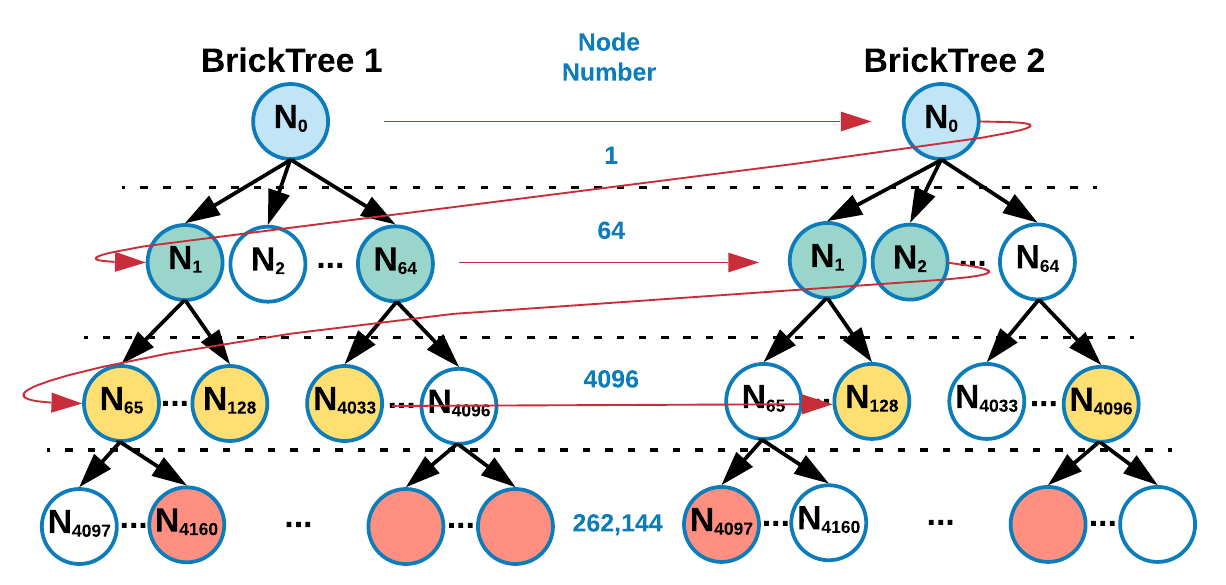
\includegraphics[width=0.5\textwidth]{LoadByLevel}
    \caption{\label{fig:loadbylevel}An illustration of streaming the Valuebrick by level. Colored nodes are requested in current time. The red arrow indicates the loading sequence.}
    %\vspace{-1em}
\end{figure}




\begin{figure*}[t]
    \centering
    \begin{subfigure}[b]{0.85\columnwidth}
        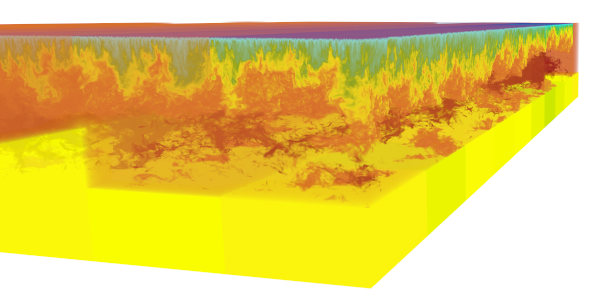
\includegraphics[width=\textwidth]{streambytree}
        \vspace{-2em}
        \caption{Stream by Bricktree}
        \label{fig:streambytree}
    \end{subfigure}
    \begin{subfigure}[b]{0.85\columnwidth}
        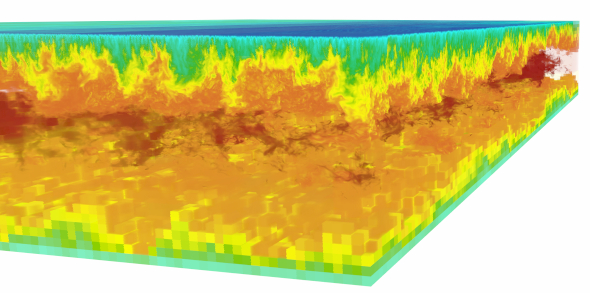
\includegraphics[width=\textwidth]{streambybrick}
        \vspace{-2em}
        \caption{Stream by Valuebrick}
        \label{fig:streambybrick}
    \end{subfigure}
    \begin{subfigure}[b]{0.85\columnwidth}
        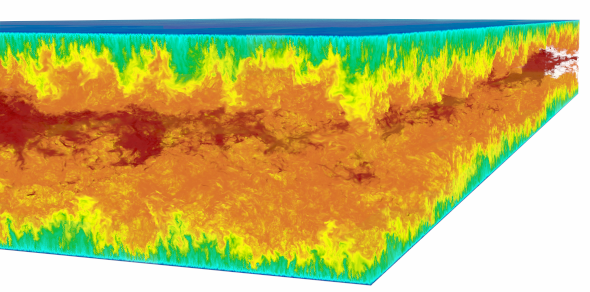
\includegraphics[width=\textwidth]{streambylevel}
        \vspace{-2em}
        \caption{Stream by tree level}
        \label{fig:streambylevel}
    \end{subfigure}
    \begin{subfigure}[b]{0.85\columnwidth}
        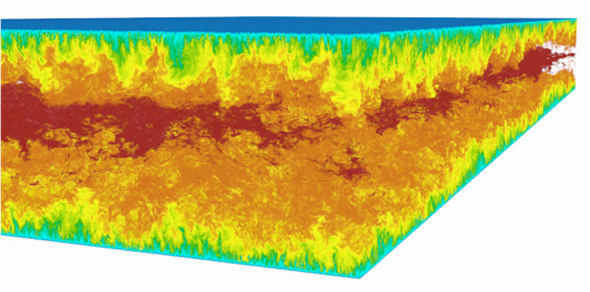
\includegraphics[width=\textwidth]{gound_truth}
        \vspace{-2em}
        \caption{Ground truth}
        \label{fig:streambylevel}
    \end{subfigure}
	\caption{\label{fig:streamstrategy}%
	A comparison of rendering images of the DNS dataset with three Valuebrick loading strategies at frame 100. Stream by level shows more detail and smoother data refinement.}
	\vspace{-0.5em}
\end{figure*}


%-------------------------------------------------------------------------
\section{Ray-Guided Progressive Rendering}
%The long waiting times of loading data from disk significantly
%influence the user experience in an interactive visualization. 
%In this section, we describe the solution to reducing IO latency with data streaming and progressive rendering. 
Benefited from the design, our Bricktree naturally leads to progressive rendering
where data streaming and rendering are decoupled in
the visualization pipeline. If the requested data are not yet in memory, the renderer uses 
the average value stored in the (already loaded) parent node
and requests the missing brick from a data loading thread. Consequently,
the visualization process can be launched very quickly without waiting for the large
data to first be loaded into the memory. In addition, rendering performance remains stable 
when the camera position is updated. 


%----------------------------------
\subsection{Valuebrick Streaming}
So far, we have illustrated how we sample and traverse the Bricktree assuming that all
multi-resolution bricks are in memory, which works well on small- or moderate-size datasets. 
For large datasets, however, IO bottlenecks and memory size limit performance and rendering
quality. In particular, IO latency for loading the dataset into memory before
rendering becomes prohibitive when visualizing large data. Loading a
terascale dataset into memory on a contemporary workstation might take hours, even with a parallel IO
library such as PIDX. Furthermore, the memory might not be adequate to load all bricks. 


To solve this problem, we employ ray-guided progressive rendering and stream bricks
on demand. Although the idea behind this approach is similar to GigaVoxel\cite{crassin2009gigavoxels}
and to Hadwiger's work \cite{hadwiger2012interactive}, our implementation on multi-core CPUs
is more straightforward, and it avoids CPU-GPU communications and the complex data structures
needed to store the rendering context. As mentioned in~\Cref{sec:bricktree_layout},
each Bricktree stores a linear array of Valuebricks. All we need to do is maintain a
status for each Valuebrick and update it correctly according to the rendering context.
In our solution, two additional bits (\textit{isRequested} and \textit{isLoaded}) are stored 
for each brick and used to identify the brick's current status. In our sample function, 
\textit{isRequested} is set when we need to load the Valuebrick
into memory, which allows us to implement a visibility-based solution that requests only
data that are inside the view frustum. 




%---------------------
\subsubsection{Progressive Sampling}
The sample function needs to be able to handle the equivalent of a cache miss -- the case
when a Valuebrick is needed but not in the memory -- to generate a correct image.
One simple and synchronous approach mentioned in \cite{crassin2009gigavoxels} is to
load the missing Valuebrick immediately and for volume integration to stop until 
the Valuebrick is loaded. 
% The implementation in the GigaVoxel paper requires costly
% CPU-GPU communication, as well as an update of a CPU-hosted backing structure.
% Although our implementation does not involve a GPU, 
This approach is problematic for interactive visualization when many Valuebricks are missing 
due to the prohibitive IO latency incurred by Valuebrick loads. Given that the inner node
in the Bricktree stores the average values of its child nodes, we adopted an
asynchronous approach for volume integration. We use the average value as an
approximation for the current sample point when we request the Valuebrick and
refine the output image when the Valuebrick is loaded in separate threads. 
\Cref{alg:sample_and_stream} depicts the pseudo-code of this process. 

\begin{algorithm}[h]
	\caption{Sampling function with progressive rendering on top of our Bricktree 
    structure}\label{alg:sample_and_stream}
	\begin{algorithmic}[1]
        \Procedure{Bt\_ISPC\_GetVoxels}{$bt, coord$}
        	\State $cBrickID\gets \textit{0}$\Comment{current brick, set to root}
            \State $pBrickID\gets \textit{$-1$}$\Comment{parent brick}
            \State \textit{\textbf{uniform} \textbf{FindStack} stack[16]}\Comment{ISPC stack struct}
            \State $stackPtr\gets pushStack(\&stack[0], cBrickID, pBrickID)$
            \While{stackPtr $>$ stack}
            	\State $--stackPtr$
                \If {stackPtr is active} 
                	\State $cBrickID \gets stackPtr.cBrickID$
                    \State $pBrickID \gets stackPtr.pBrickID$
                    \If {current brick is not requested} 
                    	\State $bt.brickStatus[cBrickID].isRequested \gets true$
                    \EndIf
                    \State
                    \If {$bt.brickStatus[cBrickID].isLoaded$} 
                		\State $childBrickID \gets getChildBrickID()$
            			\State $cOffset \gets ComputeOffset(coord)$
                		\If {$childBrickID = -1$} 
                			\State \textbf{return} value in current brick
               			\Else
                			\State $stackPtr\gets pushStack(stackPtr,childBrickID, cBrickID)$
                		\EndIf
                	\Else
                		\State \textbf{return} average value in parent brick
                	\EndIf
                 \EndIf
            \EndWhile
    	\EndProcedure
	\end{algorithmic}
\end{algorithm}

%---------------------
\subsubsection{Valuebrick Loading Strategy}
In this work, multi-threading is employed to decouple the data streaming and rendering. 
We create independent threads that are responsible for determining the streaming sequence
and loading the requested Valuebrick from the file system. These threads are able to access
the Valuebrick buffer and update the \textit{isloaded} status when a Valuebrick is loaded. 
Coordinated with the progressive sampling, an interactive and smooth visualization is achieved.

Although we achieve a stable framerate by decoupling the data streaming and rendering, the 
Valuebrick loading sequence impacts the qualitative performance of our 
progressive refinement strategy. Given the layout of our Bricktree, three choices are considered.

Recall from \Cref{sec:bricktree_layout} that the volume is encoded as a Bricktree Forest. 
Hence, the naive approach is to map the whole Bricktree into memory if a Valuebrick in the
respective Bricktree is requested. We refer to this approach as ``streaming by Bricktree''. 
This approach is easy to implement but not efficient, because Bricktrees tend to be large, 
and because many unrequested Valuebricks will be loaded. 



A finer-granularity approach is to ``stream by Valuebrick'' rather than by Bricktree. For each
Bricktree, the streaming threads will filter and load the requested Valuebricks. 
This approach yields better performance than the first approach, since loading a Valuebrick
is much cheaper than loading a Bricktree. Visually, the user will notice a smoother and finer grained refinement (as shown in \Cref{fig:streambybrick}).
However, for the first few frames, when a large number of Valuebricks are missing, performance is lackluster, since many Valuebricks will be requested at once by the ray sample function.
In the worst case, we need to load almost all Valuebricks
in the current Bricktree before moving to the next Bricktree, which results in a slight performance improvement over the first approach.



Generally, the data exploration process is ``overview first, zoom and filter, then detail-on-demand''
\cite{ferster2012interactive,wang2018association}. 
Following this mantra, 
the ideal approach is to update the data resolution progressively. 
In this work, we adopt an approach similar
to level-order tree traversal and load the requested Valuebricks by level. \Cref{fig:loadbylevel}
illustrates this approach. Given a user-defined view frustum, the streaming thread
selects the requested Valuebricks (colored) by level and pushes them into a queue to load. Due to
the large branching factor ($N^3$) of our hierarchical structure, only a small portion of the
nodes are inner nodes. For example, in \Cref{fig:loadbylevel}, using $4^3$ bricks to encode a
$512^3$ volume, only $1.6\%$ of the nodes are inner nodes. Consequently, loading the inner node levels
takes relatively little time, and we can achieve smooth visual refinement of our data. 
\Cref{fig:streamstrategy} compares visual refinement using different streaming strategies.




Another factor that improves progressive refinement performance is Valuebrick load speed,
although this is highly dependent on IO throughput. Due to the design of the Bricktree ``forest'', 
the levels of the Bricktree can be loaded in parallel, since each process is independent.
For example, we can load level 2 of tree 1 and tree 2 in parallel using $tbb::parallel\_for$. 
Compared to serial streaming, we observe that parallel streaming significantly improves performance. 


%----------------------------------
\subsection{Early Tree Traversal Termination}
So far, we have discussed a ray-guided visibility culling approach that allows our renderer
to load only the visible portion of the volume. The idea is, for a given viewport, that only part of the data
contributes to the final image. Similar ideas can be applied to improve 
rendering performance. In particular, under the right conditions, Bricktree traversal
can be stopped at an inner node that reaches the appropriate level of detail (LOD). 

%--------------------- likely to use a phrase like "camera position" or even "view position". In this sentence, I changed "viewpoint" to "view frustum" because the blocks that get loaded does not only depend on the camera position, it also depends on the camera paramete likely to use a phrase like "camera position" or even "view position". In this sentence, I changed "viewpoint" to "view frustum" because the blocks that get loaded does not only depend on the camera position, it also depends on the camera paramete likely to use a phrase like "camera position" or even "view position". In this sentence, I changed "viewpoint" to "view frustum" because the blocks that get loaded does not only depend on the camera position, it also depends on the camera paramete likely to use a phrase like "camera position" or even "view position". In this sentence, I changed "viewpoint" to "view frustum" because the blocks that get loaded does not only depend on the camera position, it also depends on the camera paramete
\subsubsection{Level-of-Detail Control}
Some primitives are smaller than the output device pixels when rendering a
large dataset at low magnification\cite{rusinkiewicz2000qsplat}. Generally, in this case,
it is hard to tell the visual difference in the interactive rendering if we use higher
resolution data. 
One general-purpose approach to reduce loading and rendering time is to store data at a discrete
level of detail and select a lower resolution LOD with primitives that more closely matches the
display resolution. 

In this work, it is easy to apply LOD-based ideas, since an inner node can be interpreted as
a coarser representation of its descendants. During traversal, we calculate the projected
screen space area of a Valuebrick and stop the traversal if the area is smaller than a 
user-defined threshold. To simplify computation, we use a sphere as an approximation of a cubic
brick. By setting the threshold to one pixel, we achieve a 2.5x speed-up when we 
zoom out and view the DNS dataset at low magnification. 


%---------------------
\subsubsection{Culling with Transfer Function}
We can stop the traversal when the Valuebrick does not contribute to the 
final image given the current transfer function. In general, the performance of interactive visualization
depends on the user-defined transfer function.
For example, the framerate drops to 2-3 fps if we make the interior of the DNS volume transparent and keep the
top and bottom boundaries opaque, because rays terminate much later
when most of the volume is transparent. Furthermore, tree traversal is still performed on each
sample even when its corresponding Valuebrick is transparent. Taking advantage of the value
range stored in each node, this can easily be avoided in our implementation. The callback
function \textit{getMaxOpacityInRange(cellRange)} allows us to look up the brick's maximum
opacity based on the current transfer function.
If the maximum opacity equals 0, the tree traversal stops at the 
current Valuebrick and skips the descendants. Although the speed-up of this optimization
depends on the data and transfer function, we achieve an average 2x speed-up for
the DNS dataset with a transparent interior.



%-------------------------------------------------------------------------
\section{Results}
In this section, we evaluate four key aspects of our system: 1) the performance of the existing OSPRay
volume renderer and our Bricktree module; 2) the performance of the Bricktree with different brick sizes;
3) data compression using the Bricktree; 4) the performance of Bricktree generation. Unless otherwise noted,
benchmarks were performed on a quad-socket workstation (FSM) with four Xeon E7-8890 v3 CPUs, with a total
of 72 physical cores at 2.5 Ghz, along with 3 TB RAM.
\feng{All test datasets are stored on a network-mounted file server over a 1Gb/s network. 
The I/O throughput of the file system is 110 MB/s.}
In the benchmark, volumes were rendered to a
$1024 \times 768$ framebuffer, and the rendering performance was measured by calculating the average framerate over 100 frames. 
\feng{Bricktree read and write bandwidths include effects from the filesystem cache, 
which may result in a measured bandwidth value that appears to exceed the underlying
hardware's capability. Nonetheless, the measured read/write times are the ones that would be observed
by a real user.}

We tested our renderer with four datasets with sizes ranging from small (e.g., magnetic 
reconnection volume\cite{guo2014formation}), to medium (e.g., the Richtmyer-Meshkov instability simulation
\cite{cohen2002three} and cardiac volume\cite{scivisdata}) to extremely large (e.g., the DNS dataset \cite{moser1999direct}).
\begin{itemize}
\item The magnetic volume, produced from kinetic simulations, is a $512^3$ float-precision dataset
(size: 512 MB) that represents magnetic reconnection in relativistic plasmas. 
\item The Richtmyer-Meshkov instability (RMI) is a simulation of carbon hexafluoride being pushed up through a wire mesh, with a resolution of $2048 \times 2048 \times 1920$ and data type of uint8 (size: 8.1 GB). It is a popular dataset and is also used in \cite{fogal2013analysis, wu2018visit, knoll2006interactive}. 
\item The cardiac volumes were obtained by way of computed tomography (CT) imaging on excised,
postmortem porcine hearts. The resolution of the data is $2048 \times 2048 \times 2612$. With a data
type of int16, the size of the data goes up to 21 GB. 
\item The DNS, produced by the Institute for Computational Engineering and Science (ICES) at the
	University of Texas-Austin, is a single $10240 \times 7680 \times 1536$ double precision volume (size: 900 GB) from a turbulent flow simulation. In our experiments, we convert it into float version (450 GB).  
\end{itemize}

\begin{figure}[h]
    \centering
    \begin{subfigure}[b]{0.9\columnwidth}
        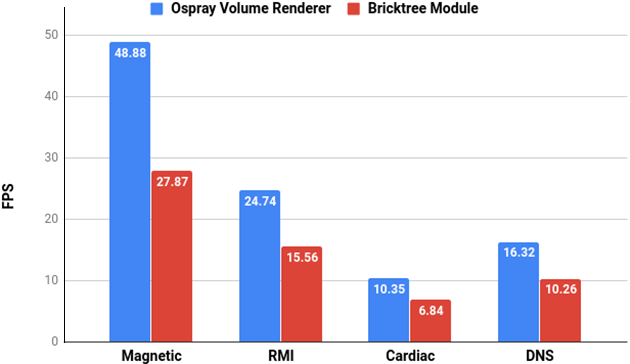
\includegraphics[width=\textwidth]{exp_ospray_bricktree_1}
        \vspace{-1em}
        \caption{Overall performance}
        \label{fig:exp_ospray_bricktree_framerate}
    \end{subfigure}
    \begin{subfigure}[b]{0.9\columnwidth}
        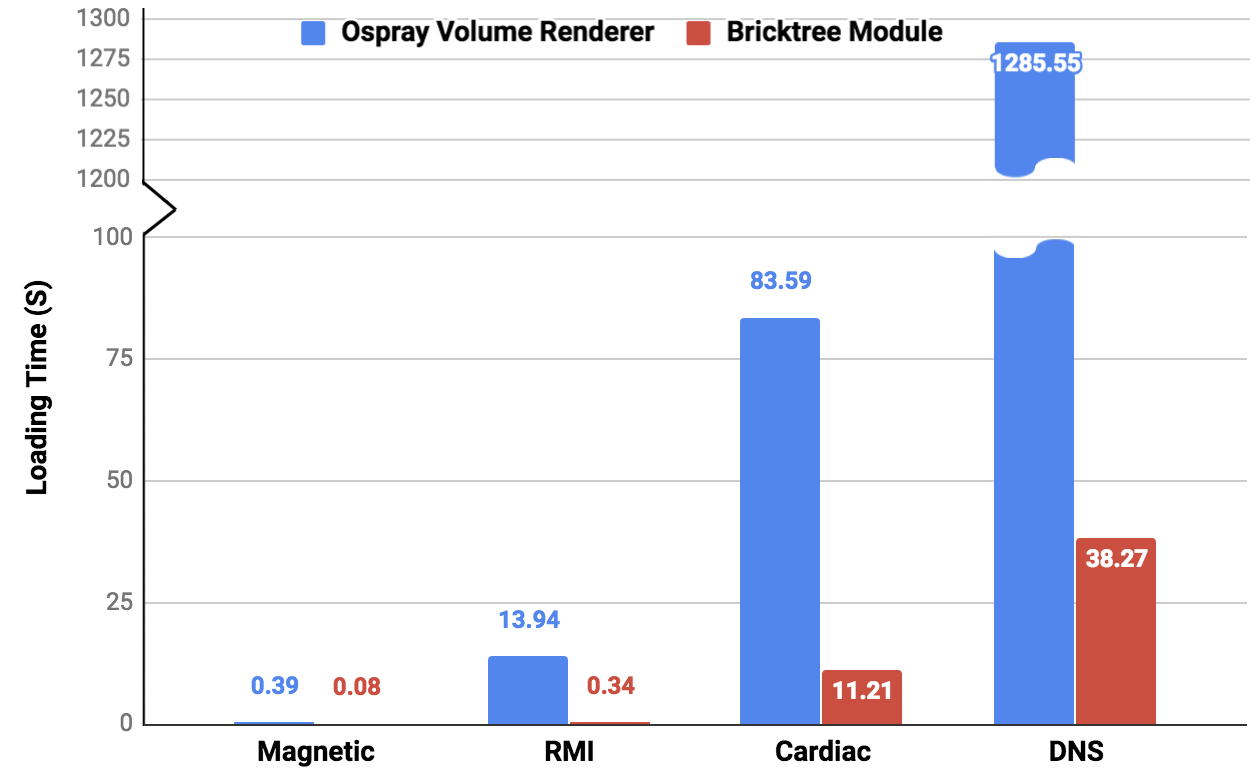
\includegraphics[width=\textwidth]{exp_ospray_bricktree_2}
        \vspace{-1em}
        \caption{Loading time before rendering the first frame}
        \label{fig:exp_ospray_bricktree_waitingtime}
    \end{subfigure}
	\caption{\label{fig:exp_ospray_bricktree}%
	A comparison of overall performance and loading time between existing OSPRay volume renderer and our Bricktree module. The evaluation was run on Bricktree with a brick size of 4.}
	\vspace{-0.5em}
\end{figure}

%----------------------------------
\subsection{Existing OSPRay Renderer vs. Bricktree Module}
%Although the existing OSPRay volume renderer provides limited support for rendering large 
%volumes on CPU, it can suffer from prohibitive IO latency, because all 
%the data must be loaded into memory before the first frame can be rendered.

\feng{
In this section, we first compare the overall performance and loading time before rendering
the first frame between our Bricktree module and the existing OSPRay volume renderer.
It is a trade-off. 
For our Bricktree module, every individual sample requires traversing a hierarchical data
structure, whereas the existing OSPRay volume renderer uses a standard structured volume and
allows data to be queried using simple math operations.
One would in fact expect each sample to be several times as costly as for the 
the reference renderer. However, given our access friendly data layout and ISPC-optimized tree
traversal, we see in \Cref{fig:exp_ospray_bricktree} that rendering performance for fully loaded 
data is only about $35\%$ slower. Despite some performance loss, 
\Cref{fig:exp_ospray_bricktree_framerate} indicates that our Bricktree module still runs
at interactive framerates.
%\Cref{fig:exp_ospray_bricktree} illustrates the trade-off between overall performance
%and loading time when volume rendering with our Bricktree module against the pre-existing
%OSPRay renderer.
%The overall performance of the Bricktree module is around $35\%$
%lower compared to the OSPRay renderer, since use of the Bricktree necessitates a hierarchy
%traversal. By contrast, the existing OSPRay renderer uses a standard structured volume
%representation, allowing data to be queried using simple math operations. 
%Despite some performance loss, \Cref{fig:exp_ospray_bricktree_framerate}
%indicates that our Bricktree module still runs at interactive framerates. 
}

\feng{
More importantly, our Bricktree module performs much better than the existing OSPRay renderer
when it comes to loading time. We measured the time that a user must wait before the renderer
draws the first frame (see in \Cref{fig:exp_ospray_bricktree_waitingtime}).
The Bricktree module achieves much better 
performance, since it needs to
load only metadata prior to rendering. With both renderers, loading time increases with
data size. However, our Bricktree module slows down much less. For instance, without
the Bricktree module, users must wait more than 20 minutes on the test workstation (FSM)
before being able to see a ``bird's eye view'' of the DNS dataset.
By contrast, with our Bricktree module, we get an overview of the DNS dataset in under 40 seconds.
%Therefore, we believe that the Bricktree module is a better choice for rendering large datasets,
%while the existing OSPRay volume renderer works better for small- to moderate-size datasets. 
}



%----------------------------------
\subsection{Choice of Brick Size}
\label{sec:exp_bricksize}

A volume renderer's domain decomposition method can have a large impact on the 
performance of the rendering pipeline\cite{fogal2013analysis}. Our design and 
implementation allow the user to easily set a custom brick size. 
We performed a set of experiments to discover how the brick size affects the
tree generation time, tree size, loading time, streaming performance and overall
framerate. Two datasets were tested: RMI (8.1 GB, int8), which is a sparse dataset, and
DNS(450 GB, float), which is a very dense dataset.

\begin{table}[h!]
	\centering
	\begin{tabularx}{\linewidth}{l*{4}{r}}
		\toprule  
		\textbf{RMI / Brick Size}   & \textbf{2} & \textbf{4} & \textbf{8} & \textbf{16}  \\
		\hline
		Tree Build (min) & 1.61 & 1.49 & 1.34 & 1.96  \\
        Tree Size (GB) & 7.80 & 5.90 & 7.10 & 9.60  \\
        Loading Time (s) & 1.48 & 0.34 & 0.15 & 0.56  \\
        Stream Performance (s) & 0.21 & 0.13 & 0.11 & 0.08  \\
        Framerate (fps) & 10.56 & 18.56 & 10.75 & 7.78  \\
		\bottomrule
	\end{tabularx}
    \begin{tabularx}{\linewidth}{l*{4}{r}}
		\toprule  
		\textbf{DNS / Brick Size}   & \textbf{2} & \textbf{4} & \textbf{8} & \textbf{16}  \\
		\hline
		Tree Build (min) & 177.22 & 92.93 & 86.66 & 80.25  \\
        Tree Size (GB) & 772 & 486 & 455 & 451  \\
        Loading Time (s) & 92.26 & 38.27 & 9.3 & 7.67  \\
        Stream Performance (s) & 0.18 & 0.16 & 0.13 & 0.08  \\
        Framerate (fps) & 15.36 & 18.38 & 36.63 & 45.62  \\
		\bottomrule
	\end{tabularx}
	\caption{An evaluation of tree build time, tree size, loading time, stream performance (s/1000 Valuebricks) and overall performance with different brick sizes on a sparse dataset (RMI) and a dense dataset (DNS). The evaluataion was run on FSM. The tree build process was executed in parallel with eight processors.}
	\vspace{-1.5em}
	\label{table:brick_size}
\end{table}

\Cref{table:brick_size} shows rendering performance with different brick sizes.
As we know, the smaller Valuebrick size is more likely to be uniform in value 
\cite{fogal2013analysis}. In our unbalanced Bricktree, a Valuebrick that contains
uniform values will not be further decomposed and stored by adopting a lossless 
fashion (mentioned in \Cref{sec:hierarchy_generation}) and setting the threshold 
to the default value (0). Under this consideration, domain decomposition with a 
small brick size is more likely to yield a Bricktree with fewer Valuebricks. 
Therefore, a small brick size is more suitable for storage and probably fast traversal. 

However, the results in \Cref{table:brick_size} indicate a slightly
different conclusion for different datasets. For a sparse dataset (e.g., RMI),
a brick size of 4 produces a smaller tree and performs better than a brick size of 8 or 16.
A brick size of 2 hampers performance and tree size, possibly due to an increased number of
inner nodes resulting from greater tree depth. 

\begin{figure}[b]
    \centering
    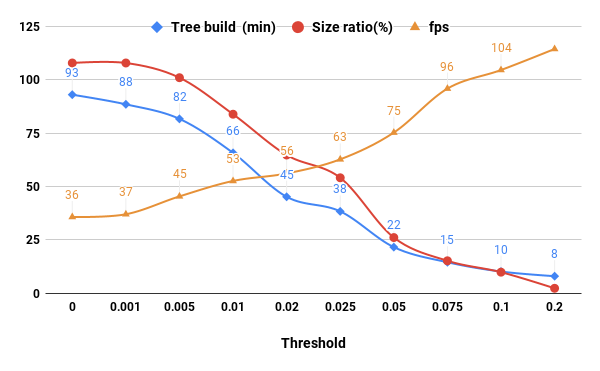
\includegraphics[width=\columnwidth]{exp_threshold}
    \vspace{-2em}
	\caption{\label{fig:exp_threshold}%
	A comparison of tree build time, size ratio (tree size / volume size) and overall performance with different thresholds on the DNS dataset.}
	\vspace{-0.5em}
\end{figure}

\begin{figure*}[t]
    \centering
    \includegraphics[width=\textwidth]{exp_threshold_2_b}
	\caption{\label{fig:exp_threshold_2}%
	A comparison of the output image rendered with four thresholds on the magnetic dataset (512~MB).
	With an appropriate threshold, such as 0.05, we achieve significant performance improvement and produce a final image that is slightly different from ground truth (thres: 0).
% 	Qualitatively, only a slight difference can be discerned in the images.
	}
	%\vspace{-0.5em}
\end{figure*}


For a dense dataset (e.g., DNS), where values vary in almost all cells,
the output Bricktree is most likely a balanced tree. Hence, we found that
a smaller brick size results in a larger tree size and longer construction time.
From the perspective of streaming performance, a large brick size is preferable 
for disk performance. For instance, the size of a Valuebrick with a
brick size 16 is 4~KB, which equals the size of a single memory page on FSM. 
Therefore, a brick size of 16 gives more a friendly memory access pattern. 
We observed that the streaming thread will influence rendering performance
when many Valuebricks are requested. For performance reasons, we believe that a 
large Valuebrick size is more appropriate for visualizing dense datasets. 
\Cref{table:brick_size} demonstrates that, for the DNS dataset, rendering
performance is the best when a brick size of 16 is used. 

\feng{Recall that a Bricktree is an octree when the brick size N is set to 2.
As shown in \Cref{table:brick_size}, a Bricktree with an appropriate 
brick size outperforms an octree in terms of framerate, tree size,
tree construction time and loading time. 
}



\subsection{Compression Results}
In ~\Cref{sec:hierarchy_generation}, we described how a threshold could be specified 
in order to collapse a specific input region of volume during the hierarchy generation.
By using the default value 0, we produced a lossless hierarchical representation of
the volume. \Cref{sec:exp_bricksize} indicates that this lossless compression
is satisfactory for a sparse dataset, since regions with uniform values
are collapsed. However, a lossy representation is generated if the threshold is
set to a positive value. ~\Cref{fig:exp_threshold} displays Bricktree build time,
the ratio of the Bricktree's size to raw volume and the rendering performance given different 
thresholds over the DNS dataset. The build time and tree size drop dramatically when 
the threshold is increased, and the rendering performance improves significantly. 
A detailed quantitative analysis of the accuracy of the output image over different 
thresholds is beyond the scope of this paper.
However, \Cref{fig:exp_threshold_2}
depicts the output image of the magnetic dataset rendered with four thresholds. Aside from the performance improvement, 
we observe that only a slight difference can be discerned in the final images if we select an appropriate threshed (e.g., 0.05) for the magnetic dataset.
On the other hand, artifacts emerge when the data are visualized with a large threshold (e.g., 0.3).
% Qualitatively, 
% there is only a slight difference in the output images.

\begin{figure}[h]
    \centering
    \begin{subfigure}[b]{0.32\columnwidth}
        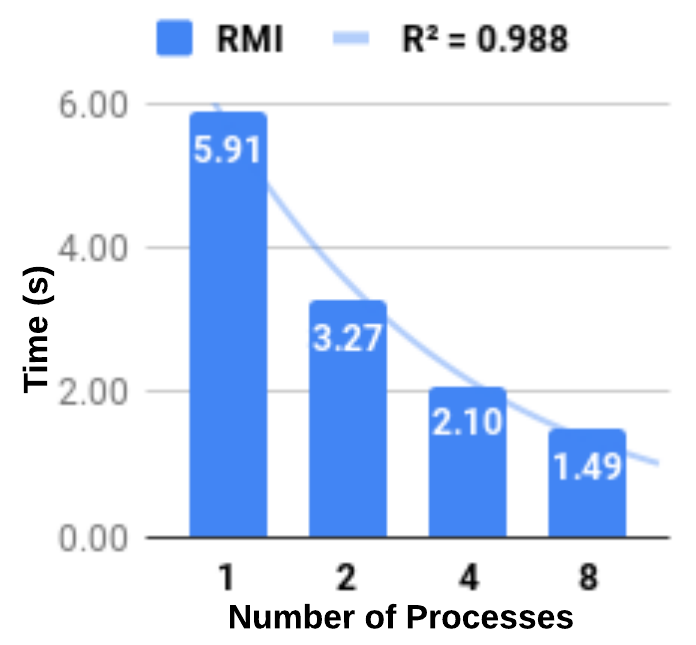
\includegraphics[width=\textwidth]{exp_buildtime_1}
        \vspace{-1.5em}
        \caption{RMI}
        \label{fig:exp_buildtime_1}
    \end{subfigure}
    \begin{subfigure}[b]{0.32\columnwidth}
        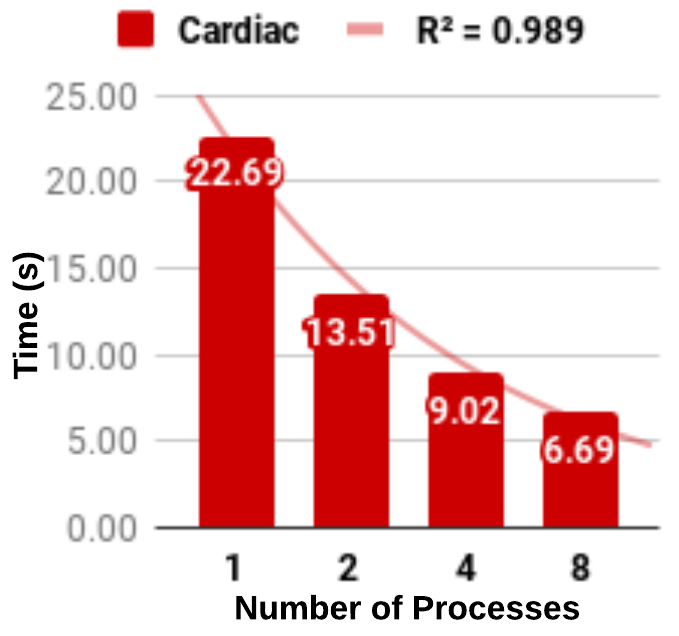
\includegraphics[width=\textwidth]{exp_buildtime_2}
        \vspace{-1.5em}
        \caption{Cardiac}
        \label{fig:exp_buildtime_2}
    \end{subfigure}
    \begin{subfigure}[b]{0.32\columnwidth}
        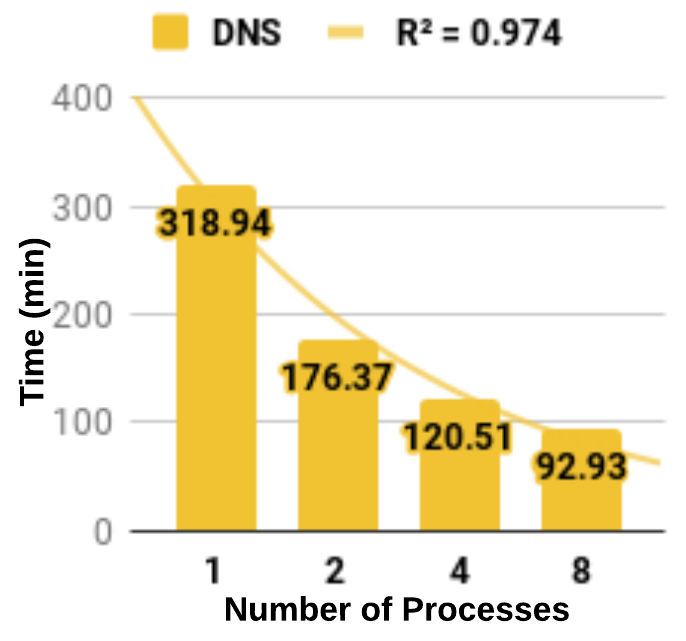
\includegraphics[width=\textwidth]{exp_buildtime_3}
        \vspace{-1.5em}
        \caption{DNS}
        \label{fig:exp_buildtime_3}
    \end{subfigure}
   
	\caption{\label{fig:exp_buildtime}%
	Tree build time by running the \textit{ospRawToBrick} tool with different numbers of processes on three datasets. The brick size of the Bricktree is set to 4 in this evaluation.}
	\vspace{-0.5em}
\end{figure}

\subsection{Bricktree Generation}

Although hierarchy generation performance has drawn less attention than rendering
performance, it is a significant bottleneck in real-world usage\cite{fogal2013analysis}. 
In this section, we evaluate the performance of the ``\textit{ospRawToBrick}'' tool. 
Tree generation time, which benefits from the parallel build processes, drops
dramatically by running multiple jobs simultaneously. \Cref{fig:exp_buildtime} shows
 hierarchy generation time with three datasets. For the RMI dataset, \cite{fogal2013analysis} claims that the generation time of their hierarchy structure takes
about 13 minutes in the best case. However, with our solution, it only takes 1.49 seconds using
eight processes. For the DNS datasets, we reduce the offline construction time from 5 hours with 
one processor to 1.5 hours with eight processors. 


\section{Conclusion}
In this paper, we have presented a solution for interactive visualization of 
large volumes on multi-core CPU architectures. Our method is based on  
hierarchical representation and ray-guided progressive rendering that 
allows the user to view and explore hundreds of gigabytes of data without
spending minutes or even hours waiting for data to load. 
Our solution is a significant improvement compared to the existing OSPRay volume renderer,
which usually takes minutes or hours to load the data prior to rendering the first frame. 
Inspired by many recent renderers, we present a hierarchical data structure
-- a Bricktree -- with a large branching factor and relatively low overhead. We have
also evaluated and discussed the tradeoffs of the different 
parameters. Based on our experimental results, we conclude that sparse datasets 
are best used with small brick sizes (e.g., 4), and dense datasets are best used with 
large brick sizes (e.g., 16). 

Our data structure naturally facilitates compression. Using the Bricktree to create an easy-to-implement lossless compression scheme, we reduced the size of the RMI dataset from 8.1~GB to 5.9~GB with a brick size of 4 
(\Cref{table:brick_size}). Furthermore, this scheme can easily be extended to support lossy compression.

Finally, we implemented our solution as a module for the OSPRay ray tracing framework. Since OSPRay is already interfaced with tools like Paraview and VisIt, users should have no difficulty putting our results into production.

%Our OSPRay module can also be leveraged by existing work integrating OSPRay into ParaView and VTK, to provide similar results to production visualization users. 

\feng{
In the future, we hope to further investigate data compression.  
For instance, Valuebricks are natural candidates for float-point data compression using ZFP
\cite{lindstrom2014fixed}. In addition, a detailed quantitative analysis of how the lossy
compression threshold affects final image quality should be performed. 
On the other hand, a hierarchical structure naturally leads to adaptive sampling. 
It is interesting to futher apply the adaptive sampling to our Bricktree module. 
Eventually, we would like to apply our Bricktree into general-purpose visualization frameworks. 
It is also interesting to look at the Bricktree structure in GPUs architecture. 
}



%-------------------------------------------------------------------------

%% if specified like this the section will be committed in review mode
\acknowledgments{
The authors wish to thank A, B, and C. This work was supported in part by
a grant from XYZ.}

%\bibliographystyle{abbrv}
\bibliographystyle{abbrv-doi}
%\bibliographystyle{abbrv-doi-narrow}
%\bibliographystyle{abbrv-doi-hyperref}
%\bibliographystyle{abbrv-doi-hyperref-narrow}

\bibliography{bricktree}

%-------------------------------------------------------------------------
\end{document}

